\documentclass[a4paper]{article}
\usepackage{latexsym,amssymb,amsmath,amsbsy,amsopn,amstext,xcolor,multicol}
\usepackage{ctex,hyperref,graphicx,wrapfig,fancybox,listings,subfigure}
\usepackage{pgf,pgfarrows,pgfnodes,pgfautomata,pgfheaps,pgfshade}
\usepackage[top=1in, bottom=1in, left=1.25in, right=1.25in]{geometry}


\setCJKsansfont[BoldFont=STHeiti]{SThei}
\graphicspath{{pic/}}
\lstset{numbers=left,
keywordstyle=\color{blue!70}, commentstyle=\color{red!50!green!50!blue!50},
frame=shadowbox,
rulesepcolor=\color{red!20!green!20!blue!20},
breaklines=true,
extendedchars=true
}

\hypersetup{
colorlinks=true,
linkcolor=black
}
\title{\bf Digital Image Processing $1^{st}$ Report}
\date{April 18 2019}
\author{生51~陈旭鹏~2014012882}

\begin{document}
\kaishu
\ttfamily
\maketitle
\tableofcontents
\newpage
%%%%%%%%%%%%%%%%%%%%%%%%%%%%%

\section{Image Fusion}
\subsection{代码说明}
本部分采取python实现,使用opencv的IO功能以及numpy, scipy的一些矩阵变换,稀疏矩阵及线性方程组求解模块。实现效果可以通过运行image fusion文件夹下的poisson\_image\_editing.ipynb文件获得。

\subsection{算法原理}
原始的泊松方程定义为:
$$
\Delta \varphi = f
$$
为了将两个图像融合,实际需要求解的方程为:
$$
\min _ { f } \iint _ { \Omega } | \nabla f - \mathbf { v } | ^ { 2 } \text { with } \left. f \right| _ { \partial \Omega } = \left. f ^ { * } \right| _ { \partial \Omega }
$$

即为了把图像source融合在图像target上,f表示融合的图像result,f*表示target image,v表示source image的梯度,$\nabla f$表示f的一阶梯度,$\Omega$表示要融合的区域,$\partial \Omega$代表融合区域的边缘部分。即在target image边缘不变的情况下,求融合部分的result image,使得result image在融合部分的梯度与source image在融合部分的梯度最为接近。

对于离散的图像,源图像的梯度可表示为:
$$
\left| \Delta B _ { ( x , y ) } \right| = 4 B ( x , y ) - B ( x - 1 , y ) - B ( x + 1 , y ) - B ( x , y - 1 ) - B ( x , y + 1 )
$$

上述公式可以转化为一个差分方程:


\begin{tiny}
\begin{equation}
H ( x , y ) - \sum _ { ( d x , d y ) + ( x , y ) \in \Omega } H ( x + d x , y + d y ) - \sum _ { ( ( d x , d ) ) + ( x y ) \in \partial \Omega } A ( x + d x , y + d y ) = \sum _ { ( d x , d y ) + ( x , y ) \in ( \Omega \cup \partial \Omega ) } ( B ( x + d x , y + d y ) - B ( x , y ) )
\end{equation}
\end{tiny}

与H有关的都是未知数,求解出这些像素值即可,把求二阶梯度的公式左边看成一个$n \cdot n$矩阵A,把未知区域的H看做是$\vec x$,把已知的source image B的二阶梯度即式子右边看做是一个$n\cdot 1$列矩阵$\vec b$,那么问题的本质就是求解
$$
A \vec { x } = \vec { b }
$$

A 的每一行至多只有 5 个非零元素,并且对角线上的元素均为 4,是一个巨大的稀疏矩阵。使用Jacobi method可以解出$\vec x = A^{-1} \vec b$,即将矩阵A分解为一个对角矩阵D和上、下三角矩阵L和U,然后每一步迭代的步骤是
$$
\mathbf { x } ^ { ( k ) } = D ^ { - 1 } ( L + U ) \mathbf { x } ^ { ( k - 1 ) } + D ^ { - 1 } \mathbf { b }
$$
可以设置$X^{(0)}=0$,然后迭代足够多次即可求解出$\vec x$

\subsection{实验结果}
第一组图的原图source,mask,target如图 \ref{fig:7}所示

\begin{figure}[htp]
\centering
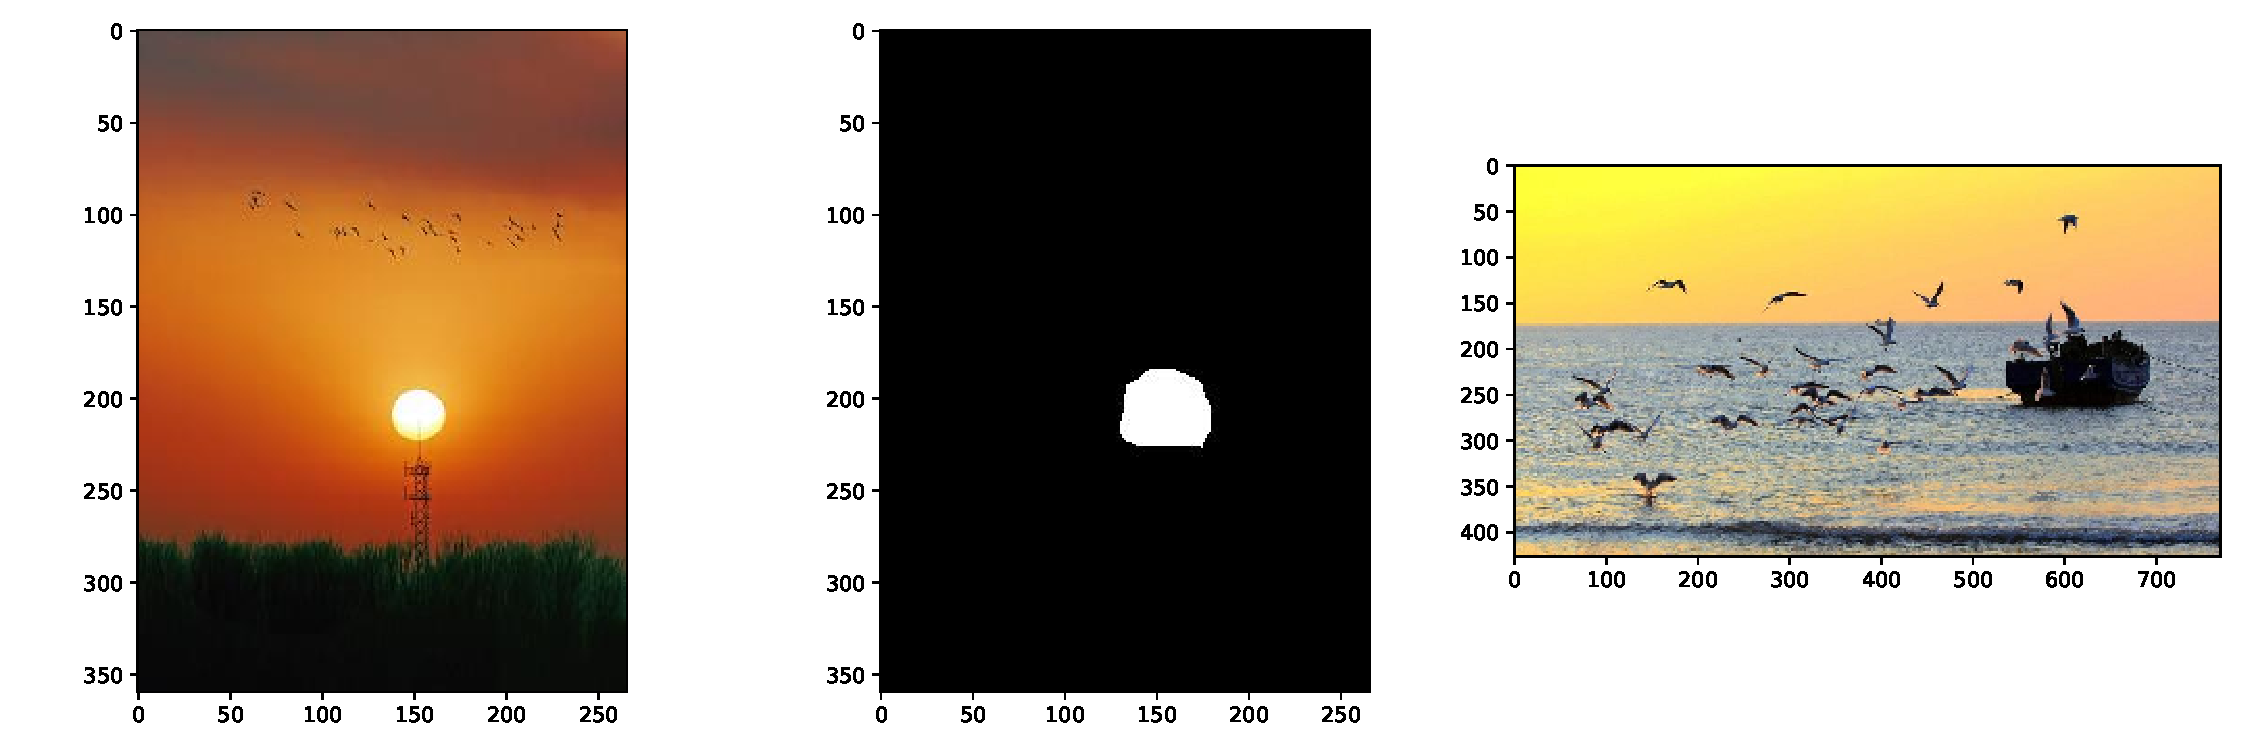
\includegraphics[width=1\linewidth]{pictures/7.pdf}
\caption{Figure 1}
\label{fig:7}
\end{figure}

融合后的图效果如图 \ref{fig:8}所示
\begin{figure}[htp]
\centering
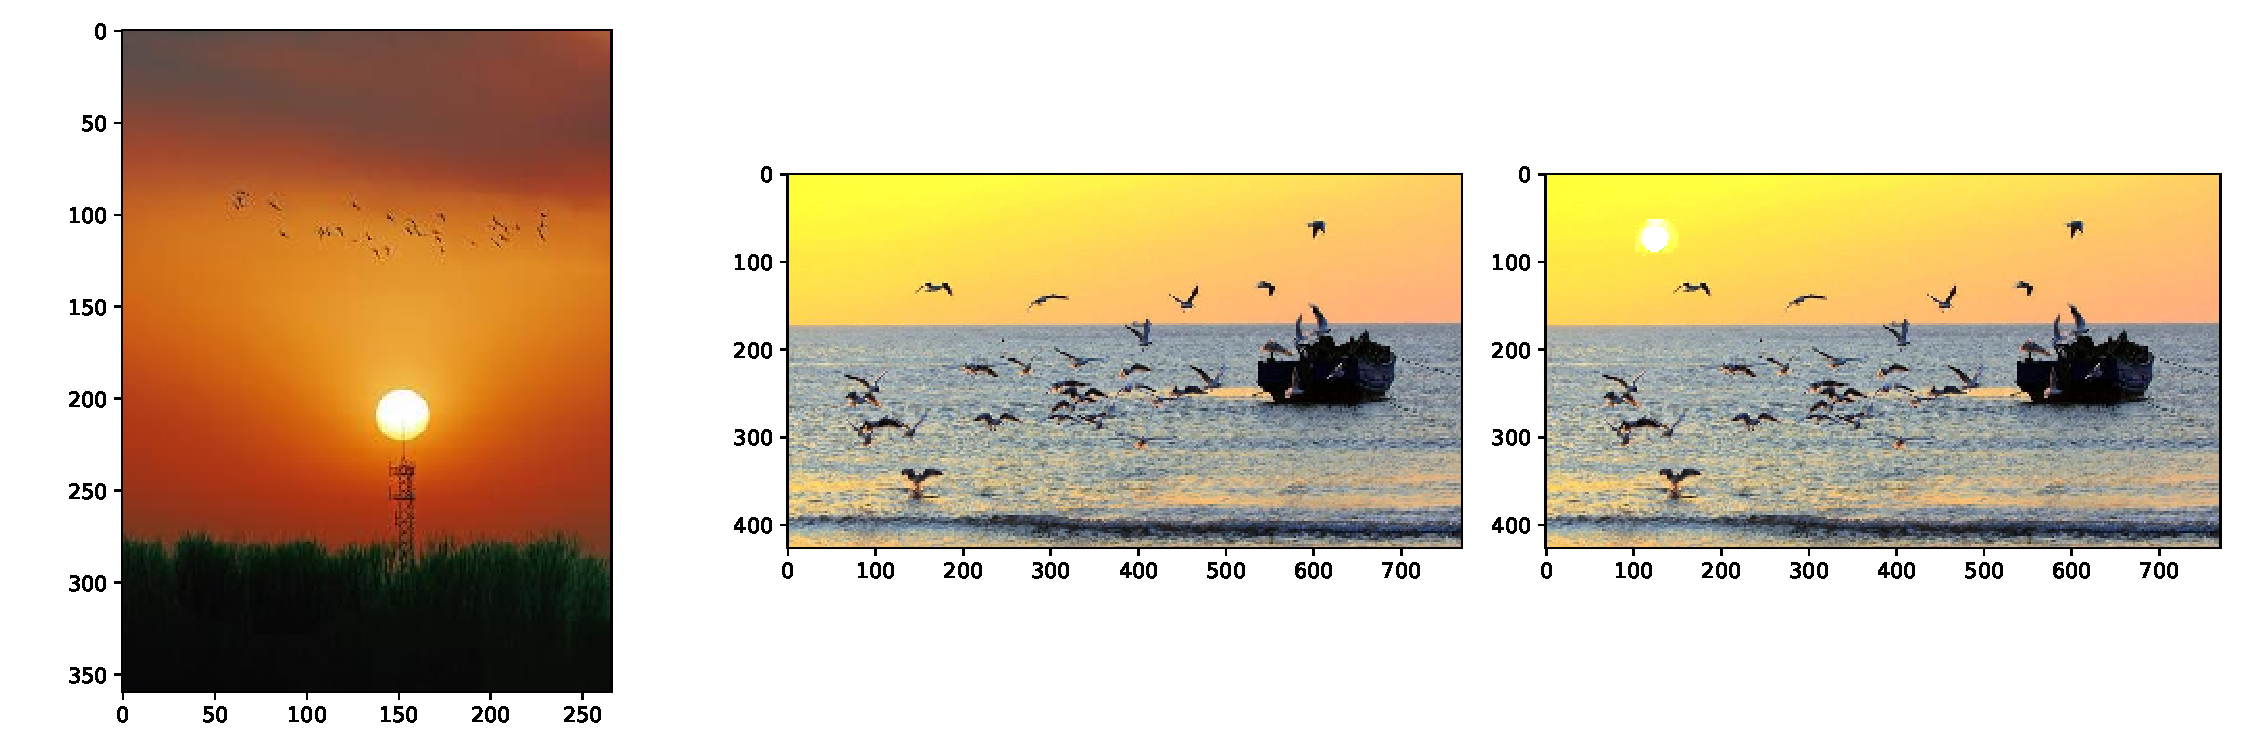
\includegraphics[width=1\linewidth]{pictures/8.pdf}
\caption{Figure 2}
\label{fig:8}
\end{figure}

第二组图的原图source,mask,target如图 \ref{fig:9}所示

\begin{figure}[htp]
\centering
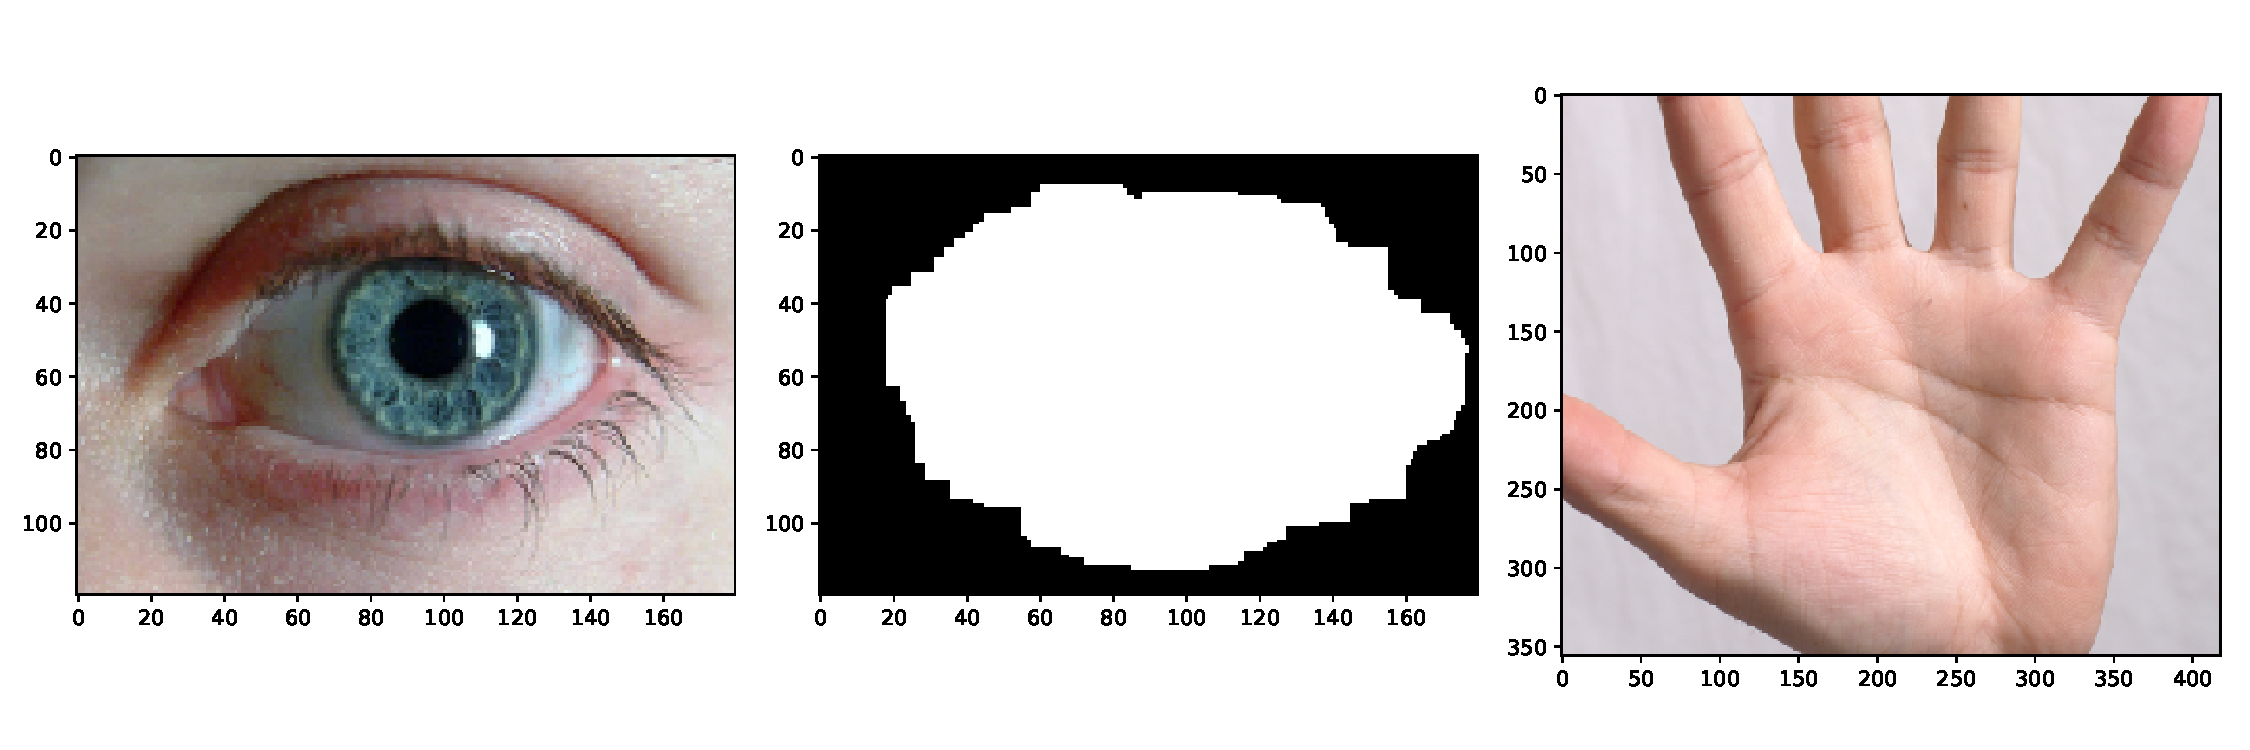
\includegraphics[width=1\linewidth]{pictures/9.pdf}
\caption{Figure 3}
\label{fig:9}
\end{figure}

融合后的图效果如图 \ref{fig:10}所示
\begin{figure}[htp]
\centering
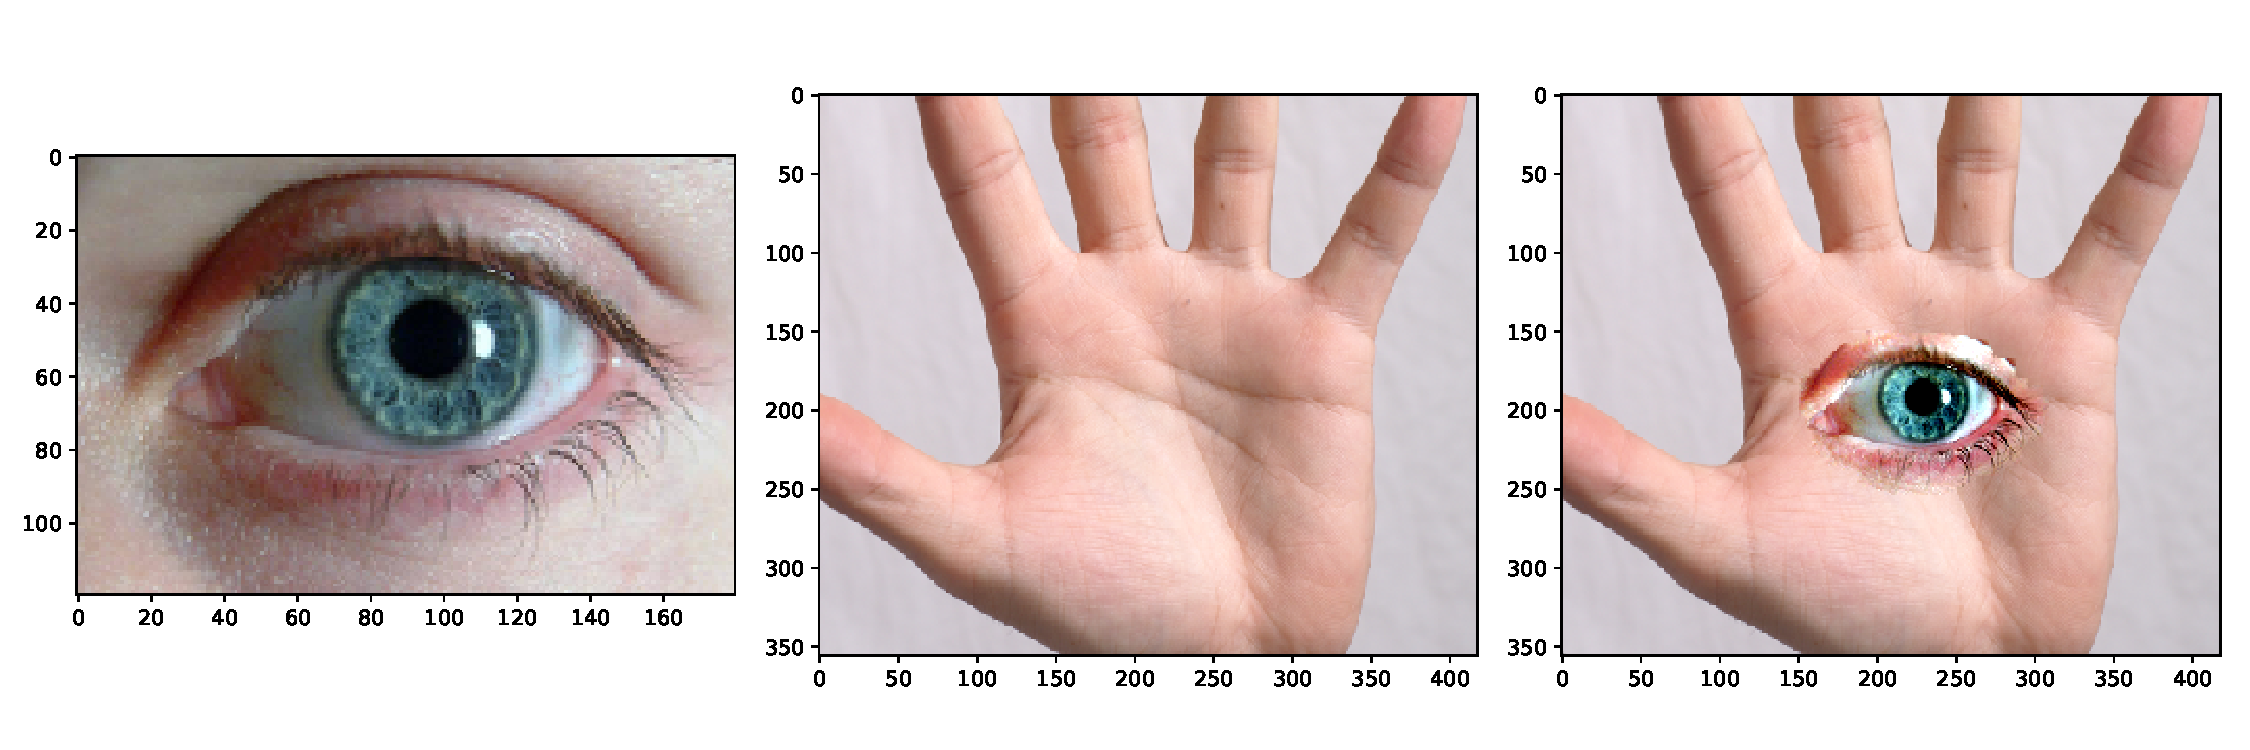
\includegraphics[width=1\linewidth]{pictures/10.pdf}
\caption{Figure 4}
\label{fig:10}
\end{figure}

虽然使用python,但是由于使用scipy的sparse和scipy.sparse.linalg.spsolve函数求解,运行时间并不是很慢,分别需要10.5和5.26s完成融合。

\section{Image Morphing}
\subsection{代码说明}
本部分采取python实现,使用opencv的IO功能以及numpy, scipy的一些函数。实现效果可以通过运行image morphing文件夹下的image\_morphing.ipynb文件获得。对于人脸的关键点检测,我调用了Face++ facepp v3 使用深度学习进行人脸的关键点检测。

\subsection{算法原理}
主要算法包括关键点检测,三角剖分,三角形的仿射变换和融合。
\begin{itemize}
\item 获取人脸的关键点即手工标注狮子面部的关键点。(由于face++不支持狮子的面部关键点标注)
\item 对于关键点进行Delaunay三角剖分
\item 对每个三角区域分别进行仿射变换并进行融合
\end{itemize} 

根据仿射变换的表达:

$$
\left[ \begin{array} { l l l } { a } & { b } & { c } \\ { d } & { e } & { f } \\ { 0 } & { 0 } & { 1 } \end{array} \right]
\left[ \begin{array} { l l l } { Source_{1x} } & { Source_{2x} } & { Source_{3x} } \\ { Source_{1y} } & { Source_{2y} } & { Source_{3y} } \\ { 1 } & { 1 } & { 1 } \end{array} \right] = \left[ \begin{array} { l l l } { Target_{1x} } & { Target_{2x} } & { Target_{3x} } \\ { Target_{1y} } & { Target_{2y} } & { Target_{3y} } \\ { 1 } & { 1 } & { 1 } \end{array} \right]
$$

其中仿射变换矩阵为:
$$
\left[ \begin{array} { l l l } { a } & { b } & { c } \\ { d } & { e } & { f } \\ { 0 } & { 0 } & { 1 } \end{array} \right]
$$
基本的矩阵求逆就可以解除affine transformation矩阵。

\subsection{实验结果}
\subsubsection{人脸关键点检测和Delaunay三角剖分}

三角剖分之后的可视化效果分别如图 \ref{fig:1},\ref{fig:2},\ref{fig:3},\ref{fig:4} 所示


\begin{figure}[htp]
\centering
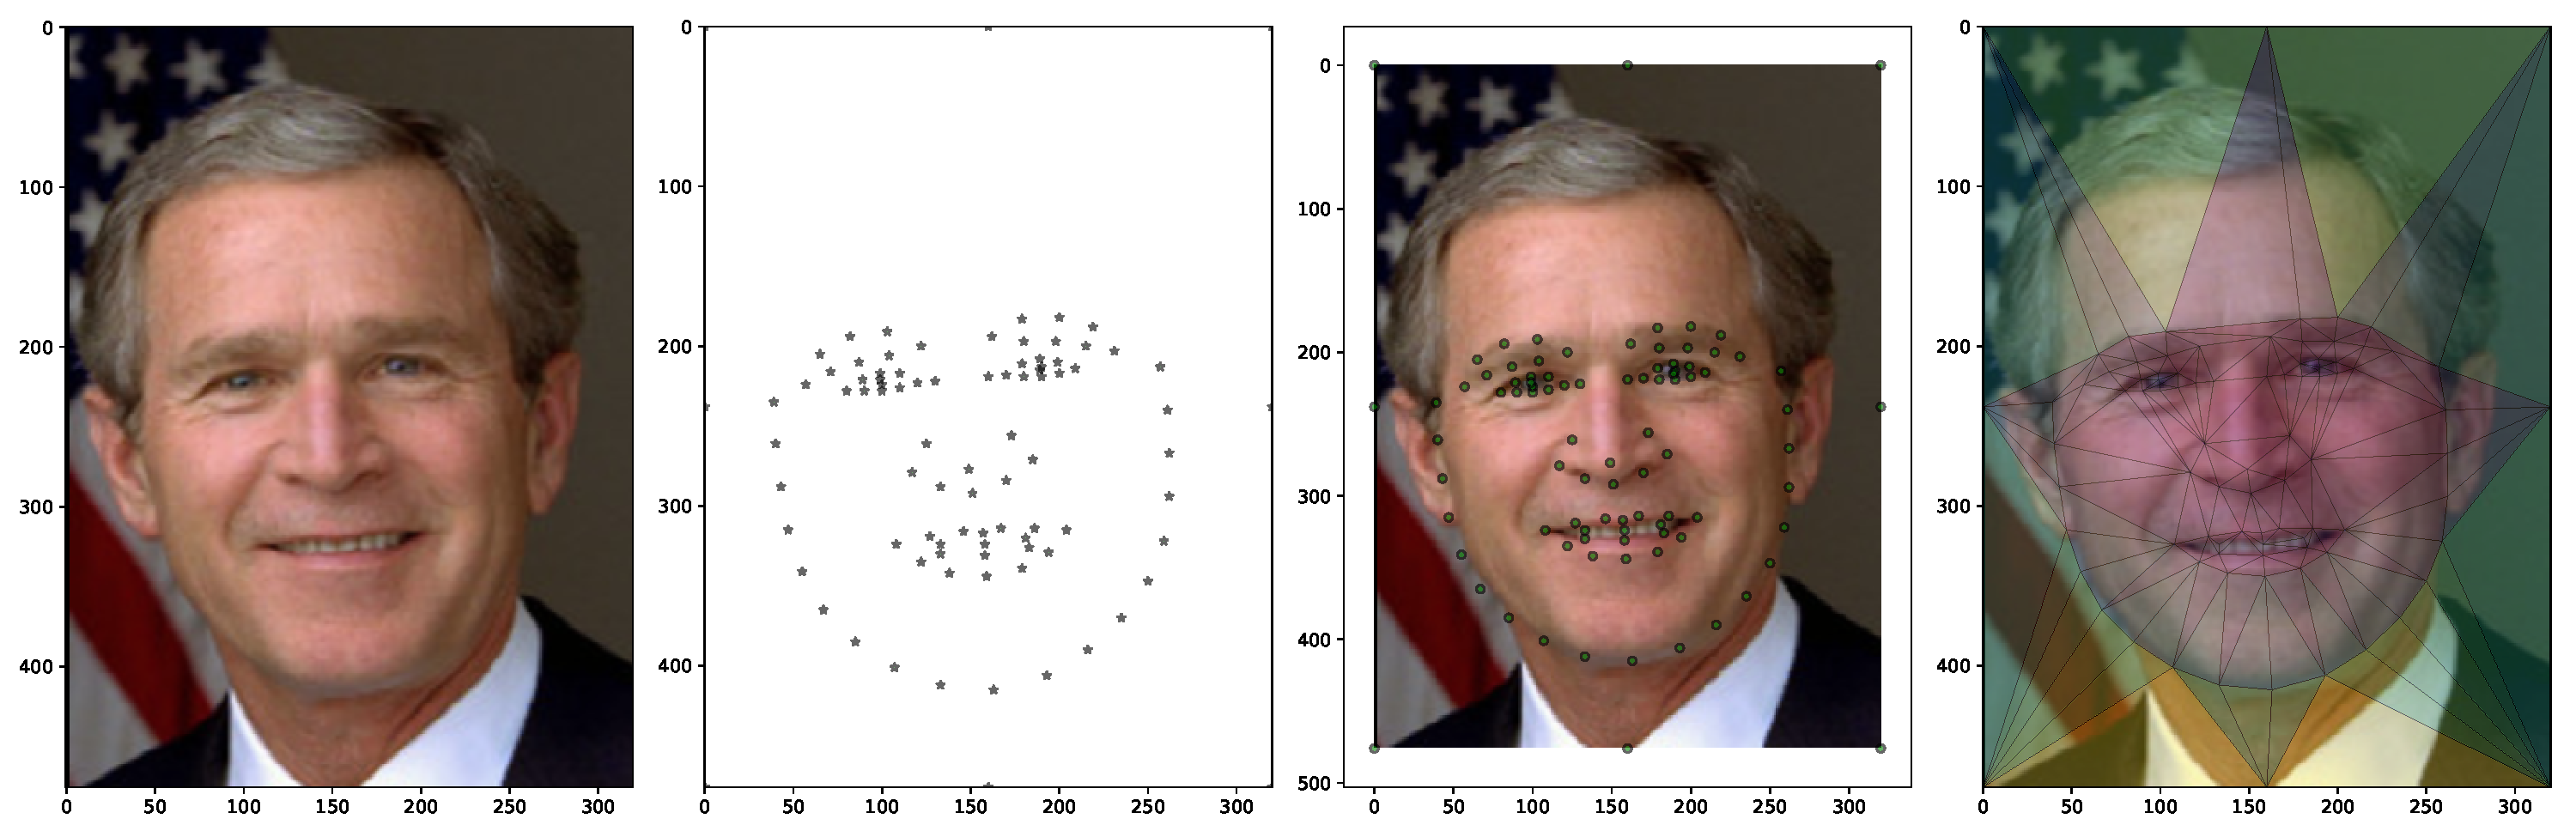
\includegraphics[width=1\linewidth]{pictures/1.pdf}
\caption{Figure 1}
\label{fig:1}
\end{figure}

\begin{figure}[htp]
\centering
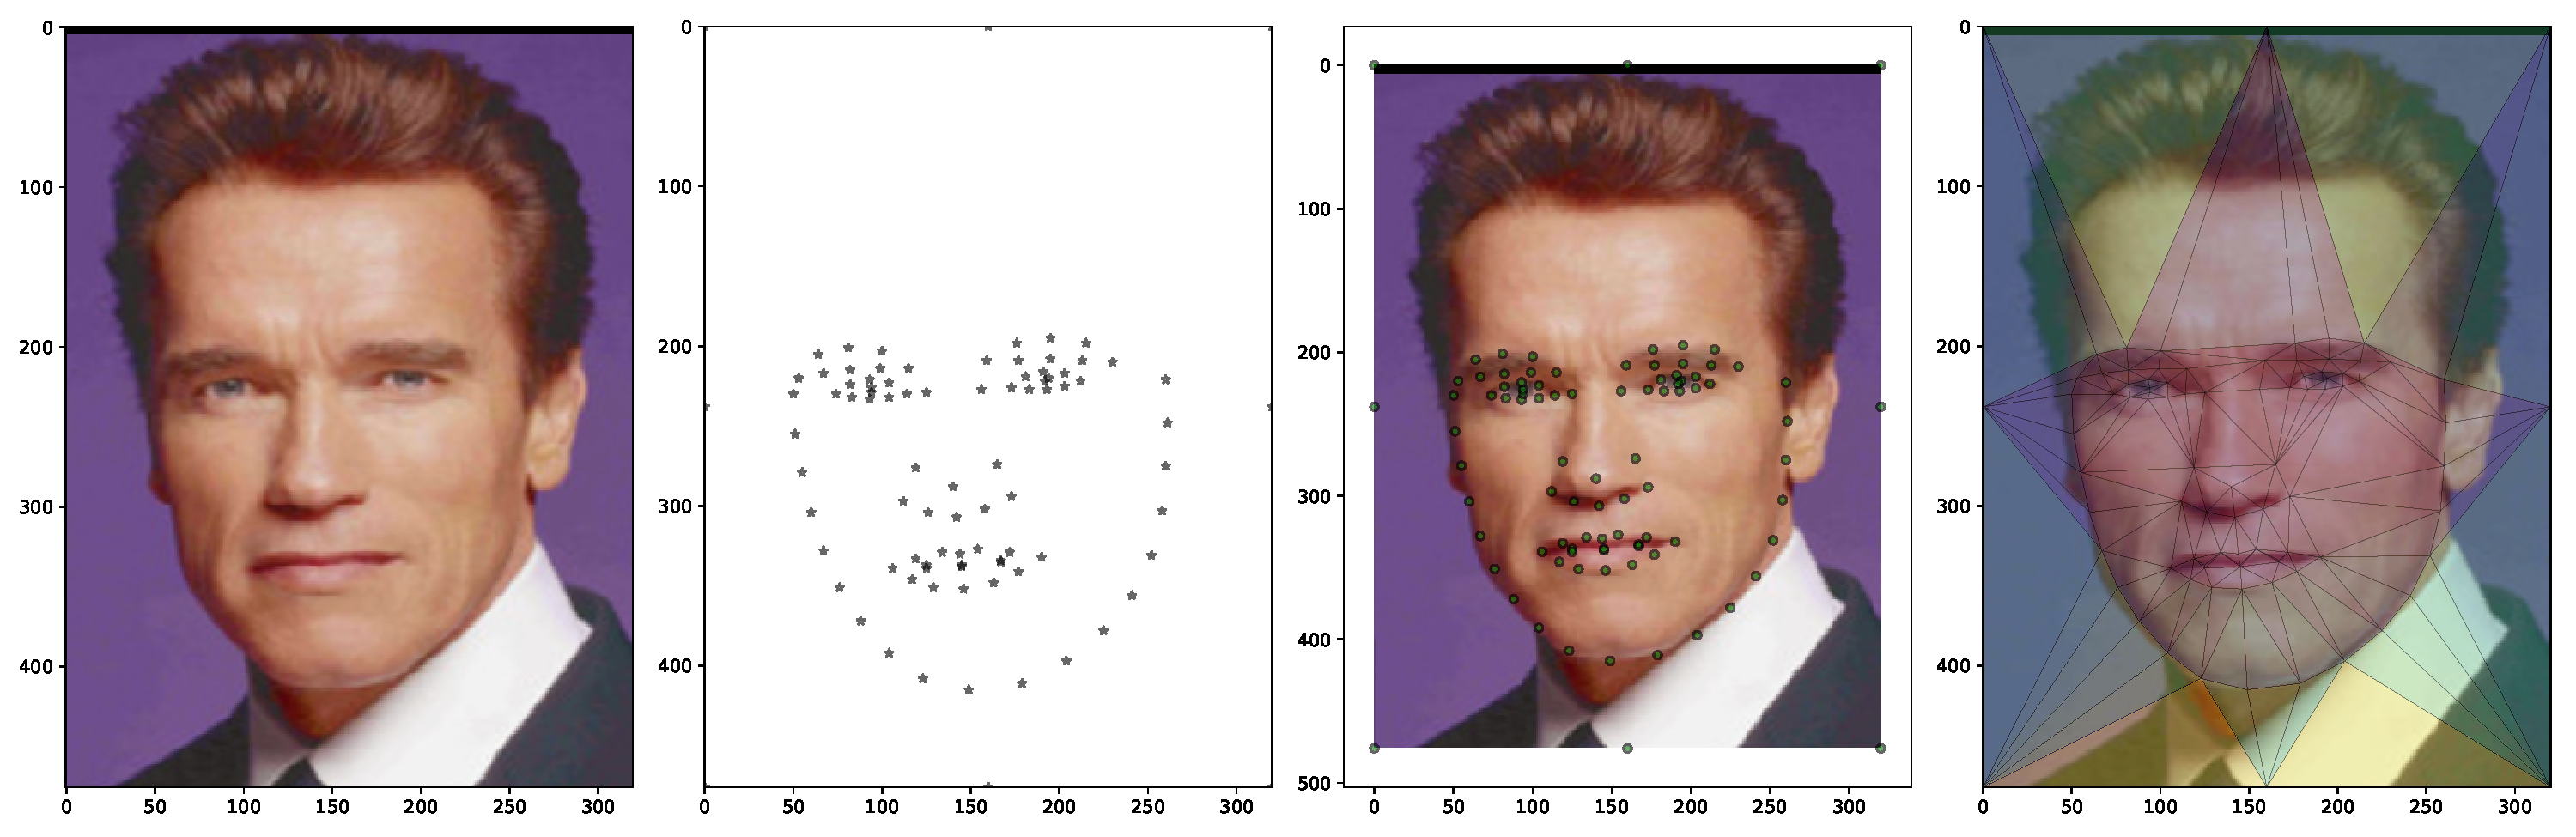
\includegraphics[width=1\linewidth]{pictures/2.pdf}
\caption{Figure 2}
\label{fig:2}
\end{figure}

\begin{figure}[htp]
\centering
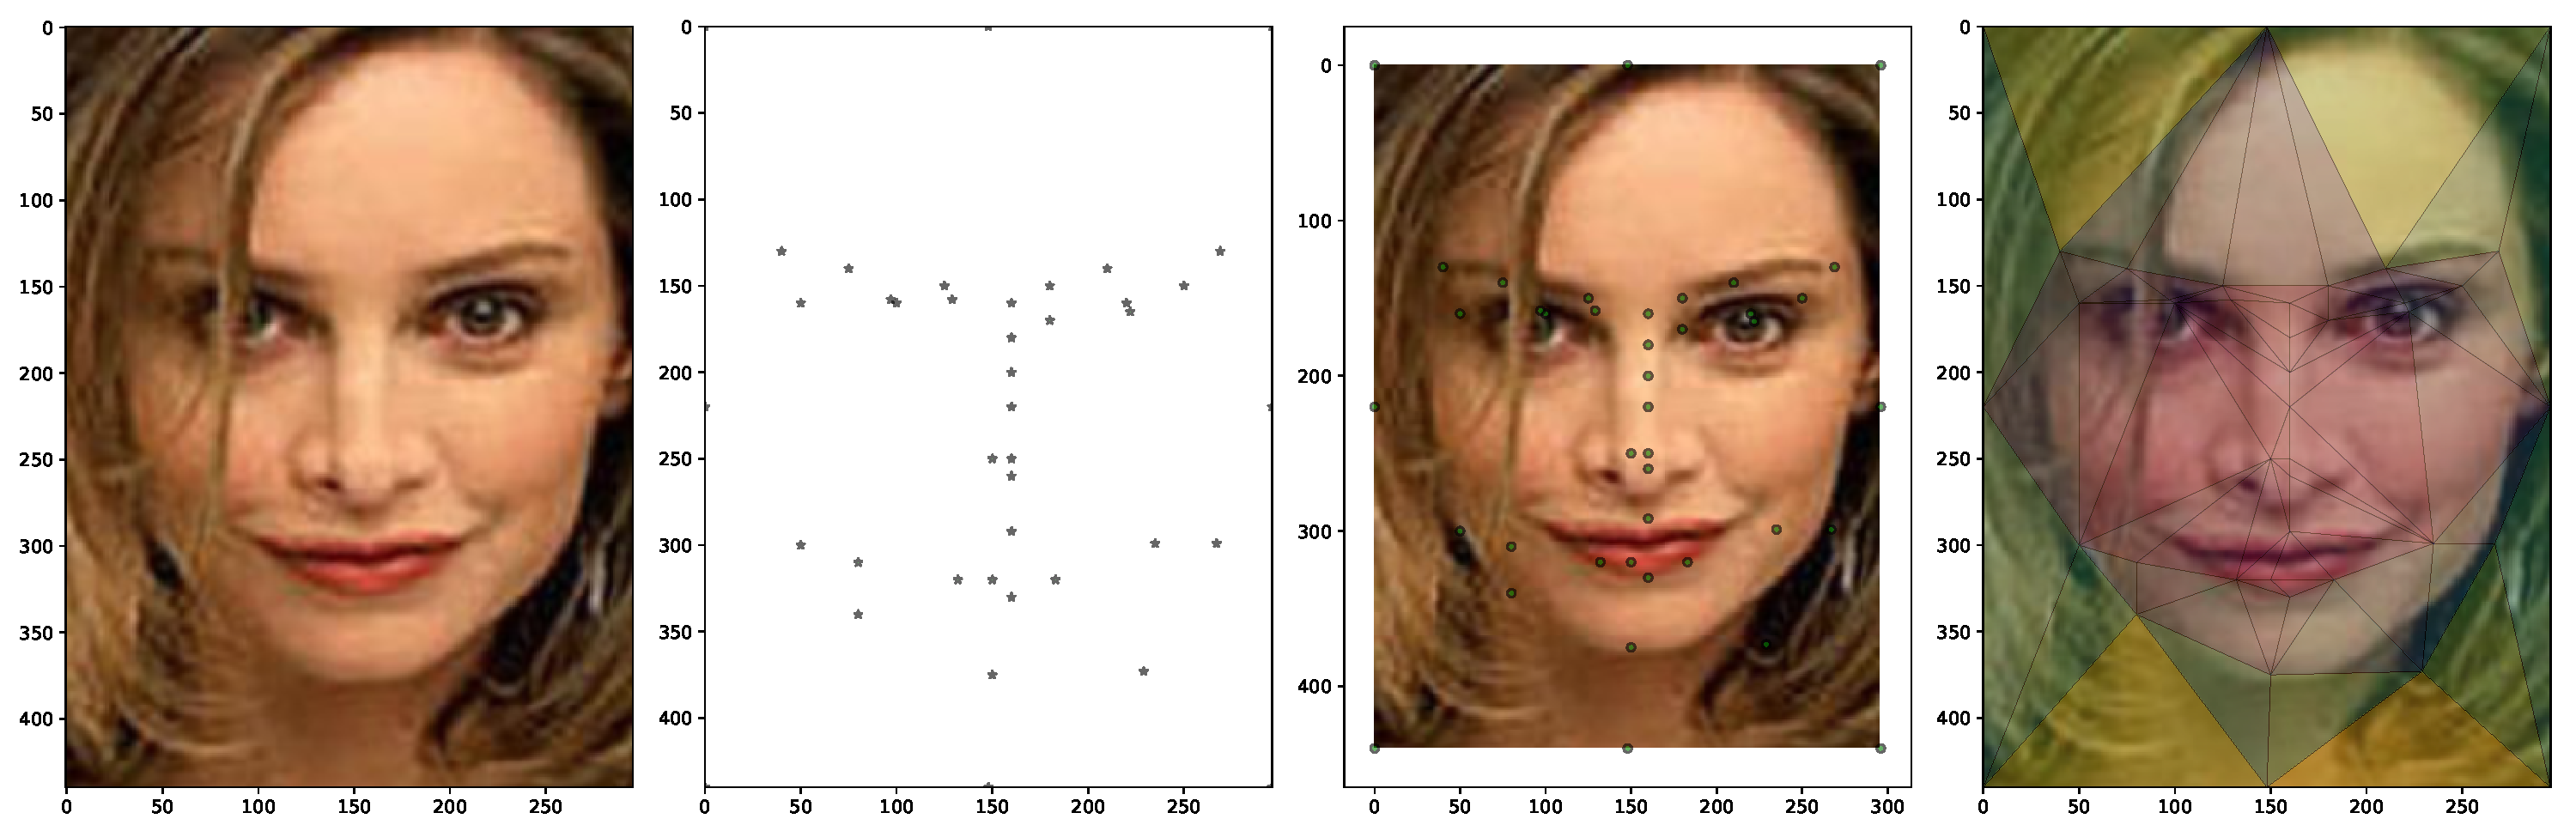
\includegraphics[width=1\linewidth]{pictures/3.pdf}
\caption{Figure 3}
\label{fig:3}
\end{figure}

\begin{figure}[htp]
\centering
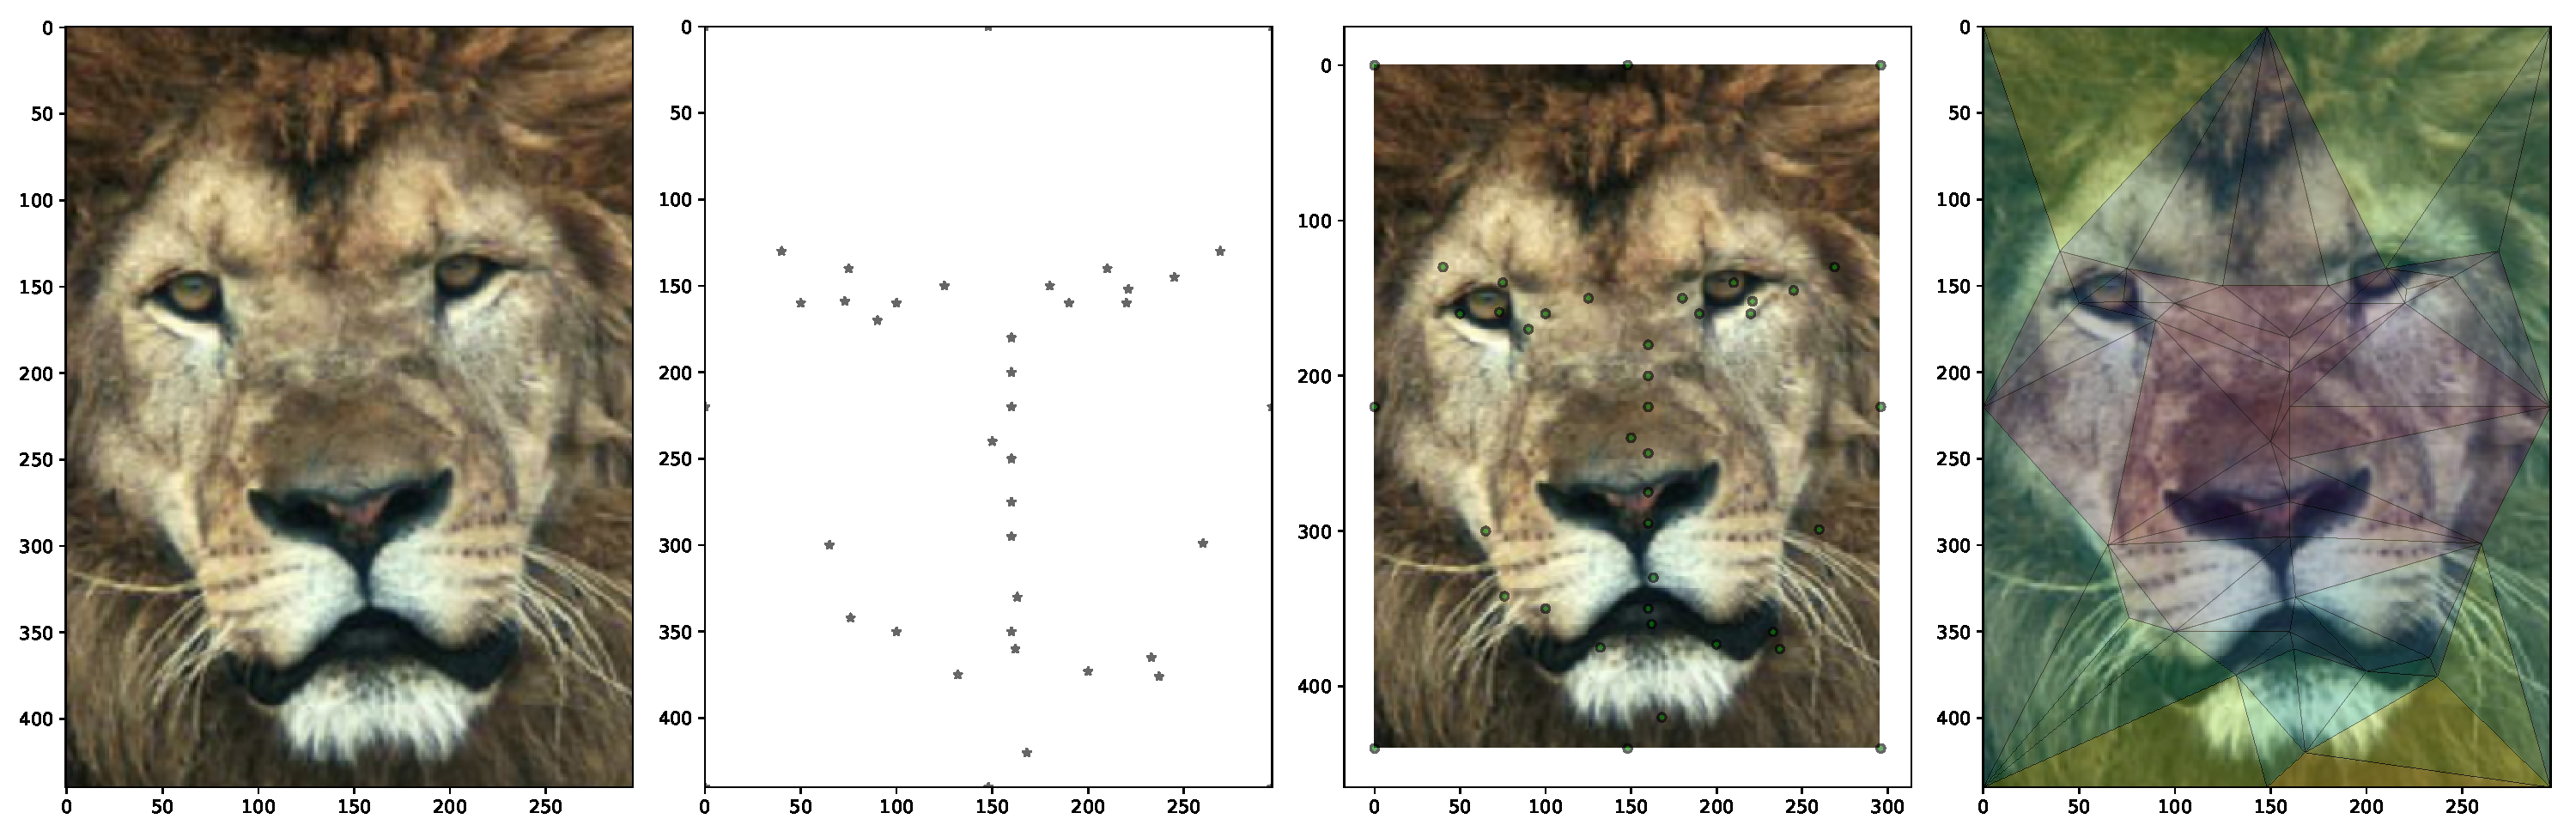
\includegraphics[width=1\linewidth]{pictures/4.pdf}
\caption{Figure 4}
\label{fig:4}
\end{figure}

\subsubsection{morphing and blending}
使用仿射变换的方法对每组三角形进行仿射变换,再按照一定的$\alpha$确定混合程度即可获得两张脸进行融合的效果。融合后的效果图如 \ref{fig:5},\ref{fig:6} 所示

\begin{figure}[htp]
\centering
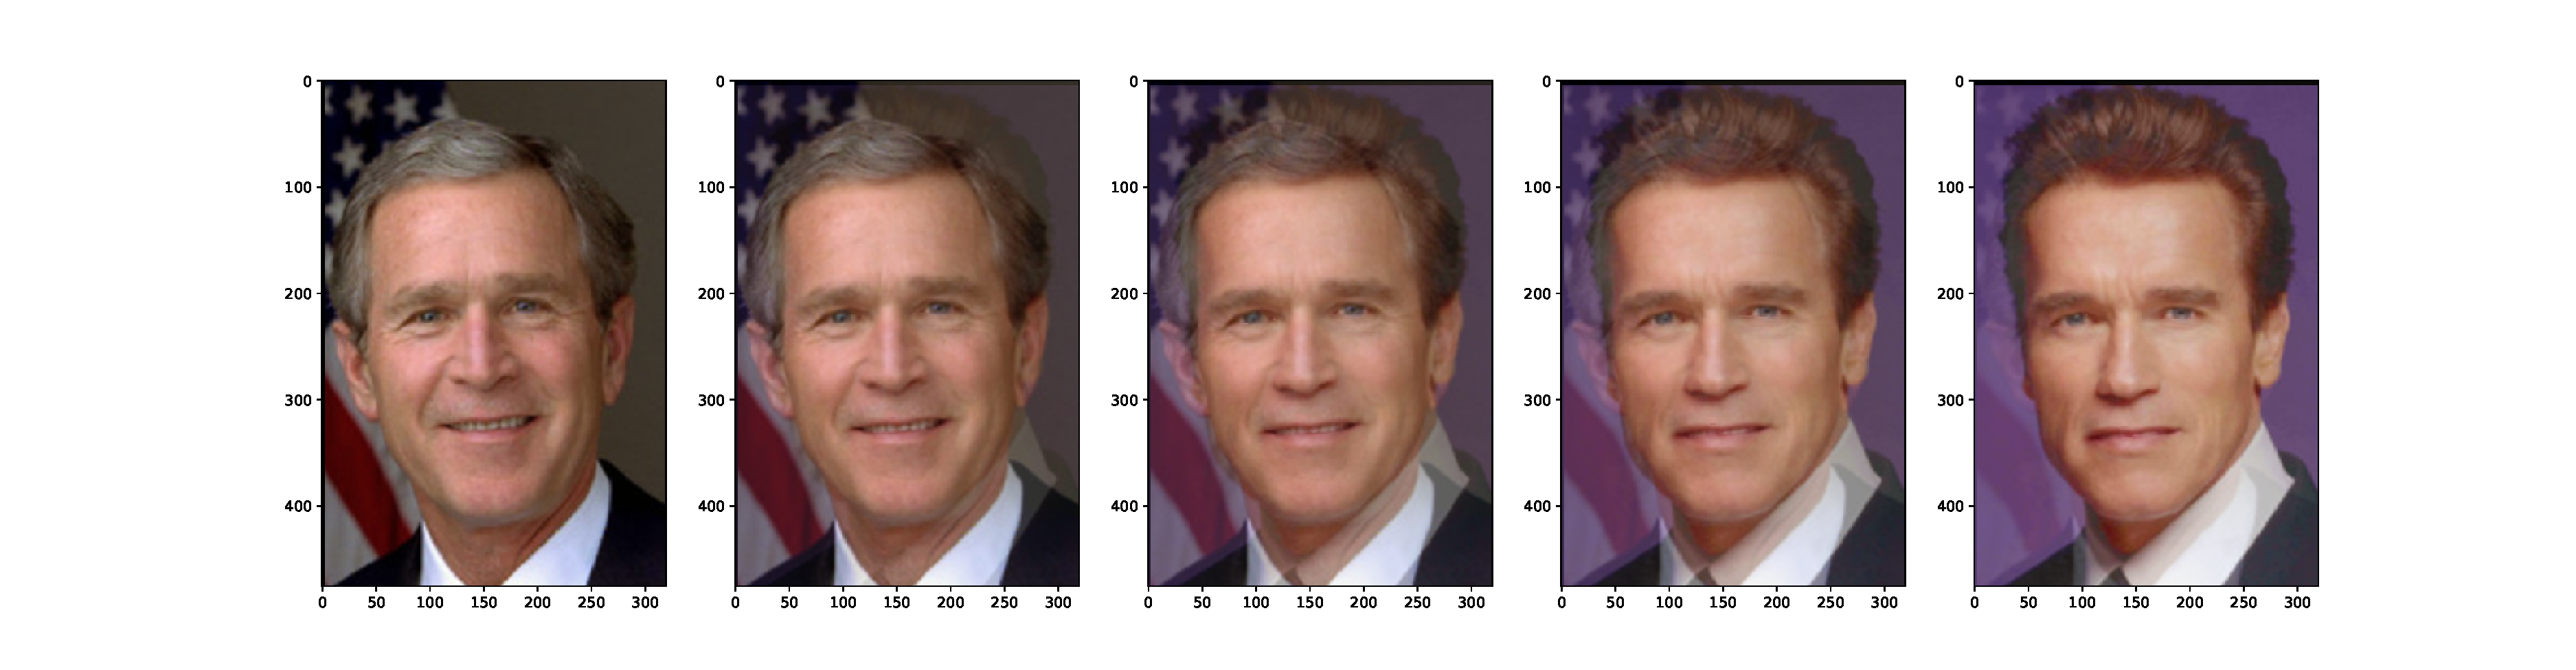
\includegraphics[width=1\linewidth]{pictures/5.pdf}
\caption{Figure 5}
\label{fig:5}
\end{figure}

\begin{figure}[htp]
\centering
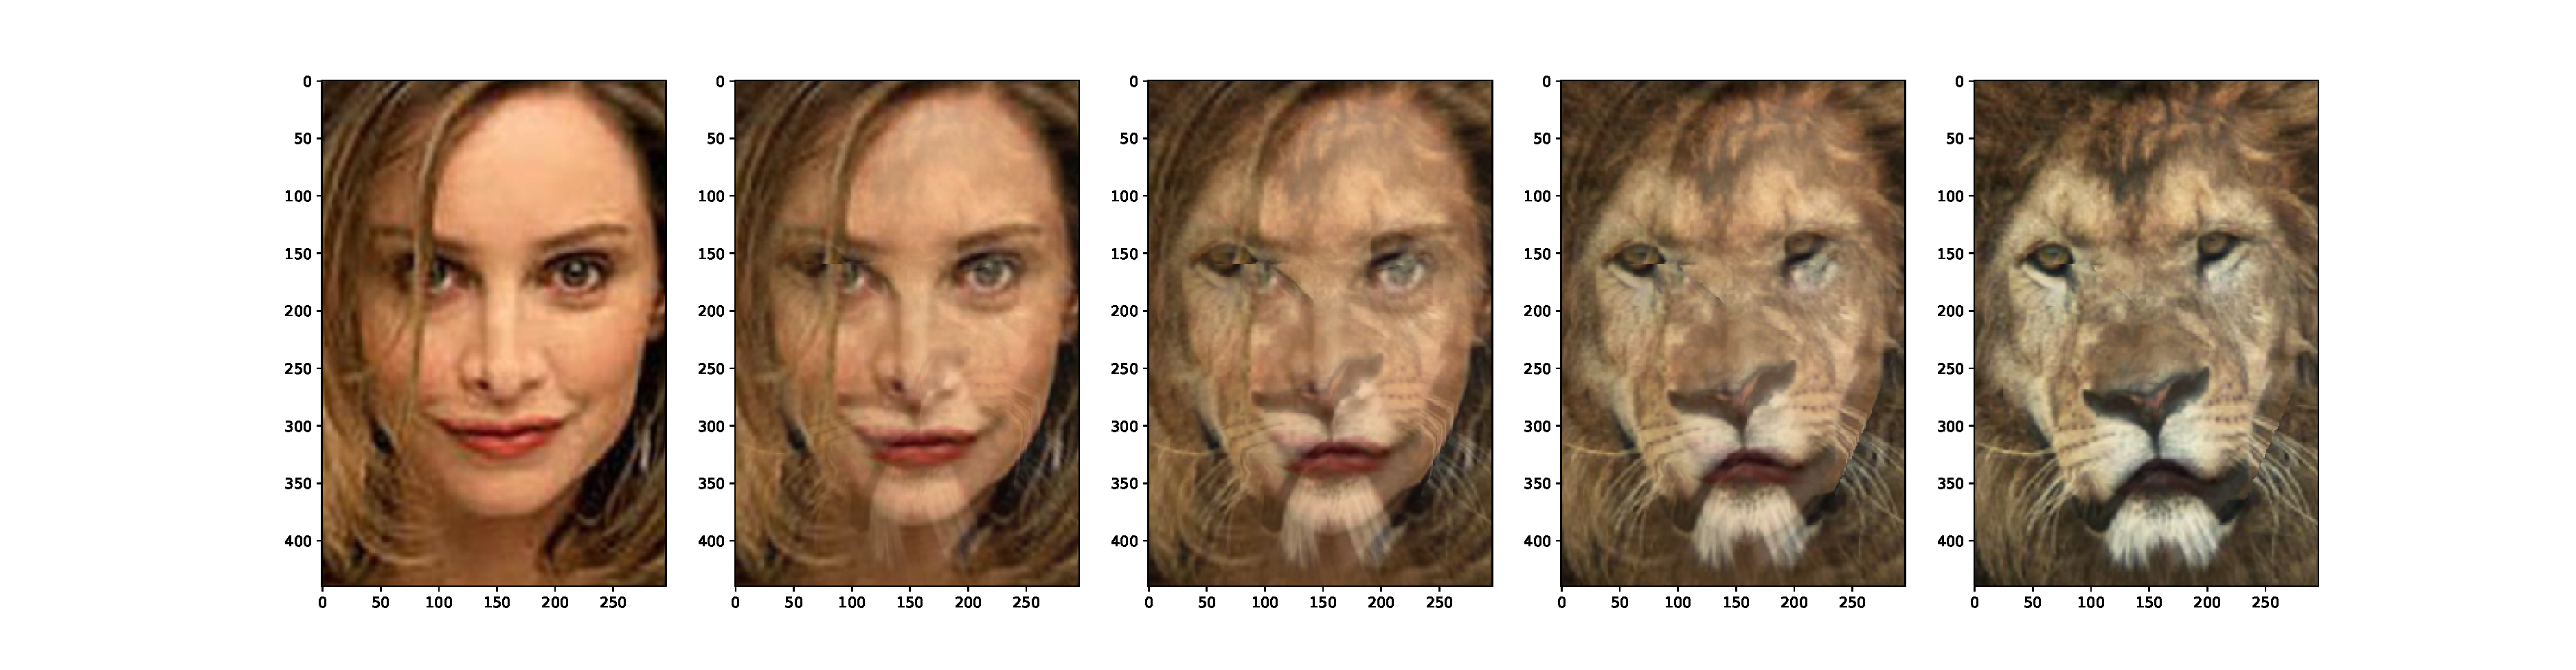
\includegraphics[width=1\linewidth]{pictures/6.pdf}
\caption{Figure 6}
\label{fig:6}
\end{figure}

值得注意的是,由于人脸和狮子脸的pattern具有较大的差异,直接的融合可能导致一些问题,因此在做关键点标注的时候,我尽可能地找到两张脸位置比较近似的点作为成对的关键点进行标注。

\section{参考文献}


[1] Patrick Pérez, Michel Gangnet, and Andrew Blake. Poisson image editing. ACM Transactions on graphics (TOG), 22(3):313--318, 2003. 

[2] Jacobi method. https://en.wikipedia.org/wiki/Jacobi\_method. 

[3] Jacobi method. http://mathworld.wolfram.com/JacobiMethod.html 

[4] Satya Mallick. https://www.learnopencv.com/face-morph-using-opencv-cpp-python/ 
%\href{https://www.learnopencv.com/face-morph-using-opencv-cpp-python/ }{Face morph using opencv}

[5] Christopher J. Tralie. Poisson image editing. http://www.ctralie.com/ Teaching/PoissonImageEditing/ 

[6] Discrete Poisson Equation https://en.wikipedia.org/wiki/Discrete\_Poisson\_equation


\end{document}
